\section{Przykłady grafów} \label{sec:common-graphs}

\subsection*{Graf pusty}

\textbf{Graf pusty} to graf, którego zbiór krawędzi jest zbiorem pustym. Każdy wierzchołek grafu pustego jest wierzchołkiem izolowanym. \blockquote{Grafy puste nie są zbyt interesujące}\footcite[30]{wilson}.

\begin{figure}[h]
\centering
\begin{tikzpicture}
\filldraw 
(0,1) node(1){}
(1,1) node(2){}
(1,2) node(3){}
(0,2) node(4){};
\end{tikzpicture}
\captionsetup{justification=centering}
\caption{Przykład grafu pustego mającego cztery wierzchołki} \label{fig:empty-graph-example}
\end{figure}

\subsection*{Graf pełny}

\textbf{Graf pełny} to graf prosty, którego każda para różnych wierzchołków jest połączona krawędzią. Graf pełny mający $n$ wierzchołków (oraz $\frac{n(n-1)}{2}$ krawędzi) oznacza się symbolem $K_n$. 

\begin{figure}[h]
\centering
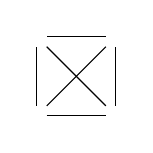
\begin{tikzpicture}
\filldraw 
(0,1) node(1){}
(1,1) node(2){}
(1,2) node(3){}
(0,2) node(4){};
\path[draw] (1)--(2);
\path[draw] (1)--(3);
\path[draw] (1)--(4);
\path[draw] (2)--(3);
\path[draw] (2)--(4);
\path[draw] (3)--(4); 
\end{tikzpicture}
\captionsetup{justification=centering}
\caption{Przykład grafu $K_4$} \label{fig:complete-graph-example}
\end{figure}

\subsection*{Graf regularny}

\textbf{Graf regularny} to graf, w którym każdy wierzchołek ma ten sam stopień. Jeśli każdy wierzchołek ma stopień $r$, to graf nazywa się \textbf{grafem regularnym stopnia $r$} (lub \textbf{grafem $r$-regularnym})\footcite[31]{wilson}. Przykładem grafu regularnego stopnia 3 jest \textbf{graf Petersena} przedstawiony na rysunku \ref{fig:petersen-graph}. Każdy graf pusty jest grafem $0$-regularnym, a graf pełny $K_n$ jest grafem regularnym stopnia $n-1$. 

\begin{figure}[h]
\centering
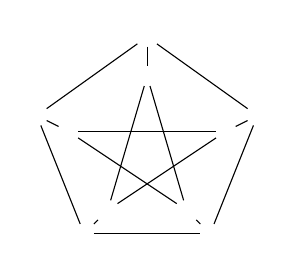
\begin{tikzpicture}
\filldraw 
(1,1.5) node(1){}
(1.5,0.5) node(2){}
(2,2.2) node(3){}
(2.5,0.5) node(4){}
(3,1.5) node(5){}%
(0.6,1.7) node(6){}
(1.2,0.2) node(7){}
(2,2.7) node(8){}
(2.8,0.2) node(9){}
(3.4,1.7) node(10){};
\path[draw] (1)--(4);
\path[draw] (1)--(5);
\path[draw] (2)--(3);
\path[draw] (2)--(5);
\path[draw] (3)--(4);
\path[draw] (6)--(1);
\path[draw] (6)--(7);
\path[draw] (6)--(8);
\path[draw] (8)--(3);
\path[draw] (8)--(10);
\path[draw] (7)--(9);
\path[draw] (7)--(2);
\path[draw] (9)--(10);
\path[draw] (9)--(4);
\path[draw] (10)--(5);
\end{tikzpicture}
\captionsetup{justification=centering}
\caption{Graf Petersena} \label{fig:petersen-graph}
\end{figure}

\subsection*{Graf cykliczny, graf liniowy, koło}

\textbf{Graf cykliczny} to spójny graf regularny stopnia 2. Graf cykliczny mający $n$ wierzchołków oznacza się symbolem $C_n$. \textbf{Graf liniowy} o $n$ wierzchołkach (oznaczany symbolem $P_n$) to graf powstały przez usunięcie jednej krawędzi z $C_n$.

Graf powstający z grafu $C_{n-1}$ poprzez dodanie dodatkowego wierzchołka i połączenie go ze wszystkimi pozostałymi nazywany jest \textbf{kołem} i oznaczany jest symbolem $W_n$. 

\begin{figure}[h]
\centering
\begin{tikzpicture}
\filldraw 
(0,1) node(1){}
(1,1) node(2){}
(1,2) node(3){}
(0,2) node(4){};
\path[draw] (1)--(2);
\path[draw] (1)--(4);
\path[draw] (2)--(3);
\path[draw] (3)--(4); 
\filldraw 
(2,1) node(5){}
(3,1) node(6){}
(4,1) node(7){}
(5,1) node(8){};
\path[draw] (5)--(6);
\path[draw] (6)--(7);
\path[draw] (7)--(8); 

\filldraw 
(6,1.1) node(9){}
(6.5,2) node(10){}
(7,1.1) node(11){}
(6.5,1.45) node(12){};

\path[draw] (12)--(9);
\path[draw] (12)--(10);
\path[draw] (12)--(11); 

  \path
    (9) edge[bend left] (10)
    (10) edge[bend left](11)
    (11) edge[bend left] (9);
\end{tikzpicture}
\captionsetup{justification=centering}
\caption{Przykład grafu $C_4$, $P_4$ i $W_4$} \label{fig:cycle-graph-example}
\end{figure}

\subsection*{Grafy dwudzielne}

\textbf{Graf dwudzielny} to graf, którego zbiór wierzchołków może być podzielony na dwa rozłączne zbiory $U$ i $V$ w taki sposób, że krawędzie nie łączą wierzchołków z tego samego zbioru. 

Ponadto jeśli każdy wierzchołek ze zbioru $U$ jest połączony dokładnie jedną krawędzią z każdym wierzchołkiem ze zbioru $V$, to taki graf jest nazywany \textbf{pełnym grafem dwudzielnym}. Jeśli moc zbioru $U$ wynosi $r$, a moc zbioru $V$ wynosi $s$, to taki graf jest oznaczany symbolem $K_{r,s}$ (ma on $r+s$ wierzchołków oraz $rs$ krawędzi).

\begin{figure}[H]
\centering
\begin{tikzpicture}
\draw[lighter-gray] (0,2.5) circle [x radius=1cm, y radius=20mm];
\draw[lighter-gray] (3,2.5) circle [x radius=1cm, y radius=20mm];
\node[draw=none,label=$U$,fill=none] at (0,-0.3) {};
\node[draw=none,label=$V$,fill=none] at (3,-0.3) {};
\filldraw 
(0,1.5) node(1){}
(0,2.5) node(2){}
(0,3.5) node(3){}
(3,1) node(4){}
(3,2) node(5){}
(3,3) node(6){}
(3,4) node(7){};
\path[draw] (1)--(4);
\path[draw] (1)--(5);
\path[draw] (1)--(6);
\path[draw] (1)--(7); 
\path[draw] (2)--(4);
\path[draw] (2)--(5);
\path[draw] (2)--(6);
\path[draw] (2)--(7);
\path[draw] (3)--(4);
\path[draw] (3)--(5);
\path[draw] (3)--(6);
\path[draw] (3)--(7);
\end{tikzpicture}
\captionsetup{justification=centering}
\caption{Przykład grafu $K_{3,4}$} \label{fig:k-3-4-graph-example}
\end{figure}
